

\section{$\lambdaLVar$: Syntax and Semantics}\label{section:programming}

The syntax and operational semantics of $\lambdaLVar$ appear in Figures
\ref{f:lambdaLVar-grammar} and \ref{f:lambdaLVar-refl}, respectively.\footnote{
We have implemented $\lambdaLVar$
as a runnable PLT Redex \cite{redex-book} model, available
in the LVars repository.}
As we have noted, both the syntax and semantics are
parameterized by the lattice $D$.  The reduction relation $\parstepsto$ is defined
on \emph{configurations} $\config{S}{e}$ comprising a store and an
expression.  
%We identify any configuration in which $S = \topS$
The \emph{error configuration}, written
$\error$,
%
is a unique element added to the set of
  configurations, but 
%% it also forms an equivalence class such that for all $e$, 
%%   $\config{\topS}{e} = \error$.
we consider $\config{\topS}{e}$ to be equal to $\error$, for all expressions $e$.
The metavariable $\conf$ ranges over configurations.

Figure~\ref{f:lambdaLVar-refl} shows two disjoint sets of reduction
rules: those that step to configurations other than $\error$, and
those that step to $\error$. Most of the latter set of rules merely propagate errors along.
A new $\error$ can only
arise by way of the {\sc E-ParAppErr} rule, which represents the joining of two
conflicting subcomputations, or by way of the {\sc E-PutValErr} rule,
which applies when a $\PUT$ to a location would take 
its state to $\top$. 

The rules {\sc E-New}, {\sc E-PutVal}/{\sc E-PutValErr}, and {\sc E-GetVal} respectively express the semantics of
the $\NEW$, $\PUT$, and $\GET$ operations described in
Section~\ref{subsection:putget}.  
The incompatibility property of the threshold set argument to $\GET$ 
is enforced in the {\sc E-GetVal} rule by the $\incomp{Q}$ premise,
which requires that the
least upper bound of any two distinct elements in $Q$ must be
$\top$.

%% LK: I'm leaving this next footnote out -- now that we *have* a real
%% implementation it reads kinda silly to speculate about what one
%% ``might'' do.

%% \footnote{Although $\incomp{Q}$ is given as a premise of the
%%   {\sc E-GetVal} reduction rule (indicating that it is checked at
%%   runtime), in a real implementation the incompatibility condition on threshold sets might
%%   be checked statically, eliminating the need for the runtime check.
%%   In fact, a real implementation could forego any runtime
%%   representation of threshold sets. }  
% \rn{Would it help to have a symbol for empty OTHER than $\bot$ here?
%   (I don't know -- $\epsilon$ or $\emptyset$ or $\bot_{\mathbb{N}}$?)
%   The problem is that the way we use it in the above threshold sets, its
%   NOT the [absolute] bottom.  Rather, it signifies that one component
%   of a larger data structure is not filled in yet.}
% \lk{I think we can leave it as $\bot$---it's clear what we mean.}
The {\sc E-Put-1/E-Put-2} and {\sc E-Get-1/E-Get-2} rules allow for
reduction of subexpressions inside $\PUT$ and $\GET$ expressions until
their arguments have been evaluated, at which time the {\sc E-PutVal}
(or {\sc E-PutValErr}) and {\sc E-GetVal} rules respectively apply.
Arguments to $\PUT$ and $\GET$ are evaluated in arbitrary order,
although not simultaneously, for simplicity's sake.
However, it would be straightforward to
add {\sc E-ParPut} and {\sc E-ParGet} rules to the semantics that are analogous
to {\sc E-ParApp}, should simultaneous evaluation of $\PUT$ and $\GET$
arguments be desired.

\FigLambdaLVishGrammar

\lk{TODO: we need a new figure that's $\lambdaLVish$ but with the freezing, etc., removed.}

\subsection{Fork-Join Parallelism}\label{subsection:fork-join}


$\lambdaLVar$ has an explicitly parallel reduction semantics: the {\sc
  E-ParApp} rule in Figure~\ref{f:lambdaLVar-refl} allows simultaneous
reduction of the operator and operand in an application expression, so
that (eliding stores) the application $\app{e_1}{e_2}$ may step to
$\app{e_1'}{e_2'}$ if $e_1$ steps to $e_1'$ and $e_2$ steps to $e_2'$.
In the case where one of the subexpressions is already a value
or is otherwise unable to step (for instance, if it is
a blocked $\GET$), the reflexive {\sc E-Refl}
rule comes in handy: it allows the {\sc E-ParApp} rule to apply
nevertheless.
When the configuration $\config{S}{\app{e_1}{e_2}}$ takes a step,
$e_1$ and $e_2$ step as separate subcomputations, each beginning with
its own copy of the store $S$.  Each subcomputation can update $S$
independently, and we combine the resulting two stores by taking their least
upper bound when the subcomputations rejoin.
(Because {\sc E-ParApp} and {\sc E-ParAppErr} perform
truly simultaneous reduction, they have to address the subtle point of
location renaming: locations
  created while $e_1$ steps must be renamed to avoid name conflicts
  with locations created while $e_2$ steps.  We discuss the
  $\mathit{rename}$ metafunction 
  and other issues related to renaming in Appendix~\ref{appendix:renaming-lemmas}.)

Although the semantics admits such parallel
reductions, $\lambdaLVar$ is still call-by-value in the sense that
arguments must be fully evaluated before function
application ($\beta$-reduction, modeled by the {\sc E-Beta} rule) can occur.  We can exploit this
property to define a syntactic sugar $\LETPAR$ for {\em parallel composition}, which 
computes two subexpressions $e_1$ and $e_2$ in
parallel before computing $e_3$:
\begin{displaymath}
\begin{minipage}[b]{0.8in}
  \begin{equation*}
\begin{split}
& \LETPAR ~x = e_1 \\ 
& \letparspace ~y = e_2 \\
& \letspace \IN~e_3 
\end{split}
\end{equation*}
\end{minipage}
\begin{minipage}[b]{0.6in}
\centering
$\defeq$
\end{minipage}
\begin{minipage}[b]{1in}
\begin{equation*}
  \app{(\app{(\lam{x}{(\lam{y}{e_3})})}{e_1})}{e_2}
\end{equation*}
\end{minipage}
\end{displaymath}
\noindent Although $e_1$ and $e_2$ can be evaluated in parallel, $e_3$
cannot be evaluated until both $e_1$ and $e_2$ are values, because the
call-by-value semantics does not allow $\beta$-reduction until the
operand is fully evaluated, and because it further disallows reduction
under $\lambda$-terms (sometimes called ``full $\beta$-reduction'').
In the terminology of parallel programming, a $\LETPAR$ expression
executes both a {\em fork} and a {\em join}.  Indeed, it is common for
fork and join to be combined in a single language construct, for
example, in languages with parallel tuple expressions such as
Manticore \cite{manticore_parallel_tuples}.

Since $\LETPAR$ expresses {\em fork-join}
parallelism, the evaluation of a program comprising nested $\LETPAR$
expressions would induce a runtime dependence graph like that pictured 
in
Figure~\ref{f:series-parallel}(a).  
% LK: removing this because we just said ``in the terminology of''.
%% In the terminology of parallel
%% algorithms,
The $\lambdaLVar$ language (minus $\PUT$ and $\GET$) can
support any {\em series-parallel} dependence graph.  Adding
communication through $\PUT$ and $\GET$ introduces ``lateral'' edges
between branches of a parallel computation,
as in
Figure~\ref{f:series-parallel}(b).  This adds the ability to
construct arbitrary non-series-parallel dependency graphs, just as with 
% , expanding the class of dependence graphs supported to the same class as
 {\em first-class
  futures} \cite{beyond-nested-workstealing}.




Because we do not reduce under $\lambda$-terms,
we can sequentially compose $e_1$ before $e_2$ by writing $\letexp{\_}{e_1}{e_2}$,
which desugars to $\app{(\lam{\_}{e_2})}{e_1}$.
Sequential composition is useful for, for instance, allocating a new LVar before
beginning a sequence of  side-effecting $\PUT$
and $\GET$ operations on it.

\begin{figure}[tb]
  \centering 
%\hspace{-3.3mm}
%\includegraphics[width=3in]{figures/SeriesParallel.pdf} 
\includegraphics[width=3in,natwidth=366px,natheight=204px]{chapter2/figures/SeriesParallel.pdf} 
\caption{\footnotesize A series-parallel graph induced by parallel
    $\lambda$-calculus evaluation (a); a non-series-parallel
    graph induced by $\PUT$/$\GET$ operations (b).}
  \label{f:series-parallel}
\end{figure}



\subsection{Programming with $\PUT$ and $\GET$}\label{subsection:programming-with-put-and-get}

\rn{Perhaps it's not important, but we don't seem to specify whether
  $\userleq$ on the numeric components of the pair is an IVar style
  ordering (horizontal), or the normal $\leq$ on numbers.  It's
  potentially confusing that we use $\leq$ in the intro, but then
  never use that order again.}

For our first example of a $\lambdaLVar$ program, we choose the elements of our lattice to be
pairs of natural-number-valued IVars, as shown in 
Figure~\ref{f:lattice-examples}(b).
We can then write the following
program:
\begin{equation}
\begin{split}
& \letexp{p}{\NEW}{ \\
& \letspace \letexp{\_}{\putexp{p}{\stateset{(3,4)}}}{ \\
& \letspace \letspace \letexp{v_1}{\getexp{p}{\stateset{(\bot, n) \setsep n \in \mathbb{N}}}}{ \\
& \letspace \letspace \letspace \dots v_1 \dots}}}
\end{split}
\label{e:getSnd}
\end{equation}
This program creates a new LVar $p$ and stores the pair $(3, 4)$ in
it.  $(3,4)$ then becomes the {\em state} of $p$.  The premises of the
{\sc E-GetVal} reduction rule hold: $S(p) = (3,4)$; the threshold set $Q =
\stateset{(\bot, n) \setsep n \in \mathbb{N}}$ is a 
pairwise incompatible subset of $D$; and there exists an element $d_1 \in Q$
such that $d_1 \userleq (3,4)$.  In
particular, the pair $(\bot, 4)$ is a member of $Q$, and $(\bot,4)
\userleq (3,4)$.  Therefore,
$\getexp{p}{\stateset{(\bot, n) \setsep n \in \mathbb{N}}}$ returns
the singleton set $\stateset{(\bot,4)}$,
{which is a first-class value in $\lambdaLVar$ that can, for example, subsequently be passed to $\PUT$.}
%\rn{I like this walkthrough -- it makes it really concrete.}

Since threshold sets can be cumbersome to read, we can define some
convenient shorthands $\GETFST$ and $\GETSND$ for working with our
lattice of pairs:
\begin{align*}
\getfstexp{p} \defeq \getexp{p}{\stateset{(n, \bot) \setsep n \in
    \mathbb{N}}} \\
\getsndexp{p} \defeq \getexp{p}{\stateset{(\bot, n) \setsep n \in
    \mathbb{N}}}
\end{align*}
The approach we take here for pairs generalizes to arrays of arbitrary
size, with {\em streams} being the special case of unbounded arrays
where consecutive locations are written.

\paragraph{Querying incomplete data structures}
It is worth noting that $\getsndexp{p}$ returns a value even if the
first entry of $p$ is not filled in.  For example, if the $\PUT$ in
the second line of \eqref{e:getSnd} had been
$\putexp{p}{\stateset{(\bot,4)}}$, the $\GET$ expression would still
return $\stateset{(\bot,4)}$.  It is therefore possible to safely
query an incomplete data structure---say, an object that is in the
process of being initialized by a constructor.  
\textred{However, notice that
we {\em cannot} define a $\GETFSTORSND$ function that returns if
either entry of a pair is filled in.  Doing so would amount to passing
all of the boxed elements of the lattice in
Figure~\ref{f:lattice-examples}(b) to $\GET$ as a single threshold set,
which would fail to satisfiy the incompatibility criterion.}

\rn{This has become somewhat redundant since it has been pointed out
  elsewhere... maybe it could be axed to save a few lines.}



\paragraph{Blocking reads}

On the other hand, consider the following:
\begin{equation}
\begin{split}
& \letexp{p}{\NEW}{ \\
& \letspace \letexp{\_}{\putexp{p}{\stateset{(\bot,4)}}}{ \\
& \letspace \letspace \LETPAR ~v_1 = \getfstexp{p} \\
& \letspace \letspace \letparspace \hspace{0.62em}\_~= \putexp{p}{\stateset{(3,4)}} \\
& \letspace \letspace \letspace \IN~ \dots~v_1~\dots }}
\end{split}
\label{e:getSndWithBlock}
\end{equation}
Here $\GETFST$ can attempt to read from the first entry of $p$ before it
has been written to.  However, thanks to $\LETPAR$, the $\GETFST$
operation is being evaluated in parallel with a $\PUT$ operation that
will give it a value to read, so $\GETFST$ simply {\em blocks} until
$\putexp{p}{\stateset{(3,4)}}$ has been evaluated, at which
point the evaluation of $\getfstexp{p}$ can proceed.

In the operational semantics, this blocking behavior corresponds to
the last premise of the {\sc E-GetVal} rule not being satisfied.  In
\eqref{e:getSndWithBlock}, although the threshold set $\stateset{(n, \bot)
  \setsep n \in \mathbb{N}}$ is incompatible, the {\sc E-GetVal} rule
cannot apply because there is no state in the threshold set that is lower
than the state of $p$ in the lattice---that is, we are trying to
$\GET$ something that is not yet there!  It is only after $p$'s state
is updated that the premise is satisfied and the rule applies.

% \amr{This is really bothering me. There is no sense in operational
%   semantics in which rules only fire if certain conditions are
%   satisfied. Perhaps, the way to say in a standard way is to add
%   another reduction that steps the configuration to itself if the side
%   condition is not satisfied.}

% \lk{We actually do have such a rule.  It is the {\sc E-GetValBlock}
%   rule in Figure~\ref{f:lambdaLVar-getvalblock}.  The reason why we
%   don't have that in Figure~\ref{f:lambdaLVar-refl} is because the {\sc
%     E-Refl} rule subsumes it, so the configuration does in fact step
%   to itself.  I am honestly not sure why this isn't OK (it runs in
%   Redex, albeit slowly).}




%% \subsection{Converting from Threshold Sets to $\lambda$-terms and Back}

%% {There are two worlds that $\lambdaLVar$ values
%% may inhabit: the world of threshold sets, and the world of
%% $\lambda$-terms.  
%% %
%% % While it is possible to leave 
%% But if these worlds are disjoint---if threshold set values are opaque
%% atoms---certain programs are impossible to write.  For example,
%% implementing single-assignment arrays in $\lambdaLVar$ requires
%% that arbitrary array indices can be computed \new{(\eg, as Church numerals)} and converted to threshold sets.
%% %% For example, a $\lambdaLVar$
%% %% implementation of arbitrary-length single-assignment arrays
%% %% (I-structures) requires that integer array indices, perhaps encoded as
%% %% Church Numerals, be converted into threshold sets.}
%% }
%% {Thus we parameterize our semantics by a {\em conversion
%%     function}, $\delta : v \rightarrow v$, 
%%    exposed through the $\REIFY$ language form.
%% \new{
%%     The $\REIFY$ function is {\em arbitrary}, without any particular structure, similar
%%     to including an abstract set of primitive functions in the language.
%% }
%%   %% The conversion function can arbitrarily convert between representations of values as
%%   %% threshold sets and representations as $\lambda$-terms.
%%   It is {\em optional} in the sense that providing
%%   an identity or empty function is acceptable, and leaves $\lambdaLVar$
%%   sensible but less expressive.
%%   %% (\ie, threshold sets are still first-class values,
%%   %% but usable only for passing to $\GET$ and $\PUT$).
%%   \new{
%%     This is mainly a notational concern 
%% %   This is a concern only for the formalism
%%     that does not have significant
%%     implications for a real implementation.}
%% \if{0}
%% \footnote{A
%%     reasonable alternative definition of $\lambdaLVar$ would 
%%     remove threshold set values entirely and require that threshold
%%     set inputs and outputs to $\GET$/$\PUT$ be implicitly
%%     $\REIFY$ed.  Yet the language is deterministic even in its more
%%     general form---with first-class threshold sets---and we do not want 
%%     to unduly restrict the language.}
%% \fi{}
%% % ; no other computation can be done on them.
%% }

%% {The two most common applications of value conversion are {\em
%%     reification} and {\em reflection}.  Reification is the process of converting
%%   a threshold set returned from a call to $\GET$ into a $\lambda$-term
%%   usable by the rest of the program.
%%   A typical reification
%%   function might, for instance, convert $\stateset{(3, 4)}$ to a
%%   standard Church encoding for pairs of natural numbers.
%% % substituting a non-terminating
%% %   expression (or one that signals an error) for $\bot$.  
%% %
%% %   we could achieve the same simplification through a simple set 
%% %could always achieve this simplification by a set of conventions
%% %restricting $\lambdaLVar$.
%% }
%% Conversely, reflection constructs threshold sets 
%%   from a $\lambda$-term representation.
%%   Because of the general $v
%%   \rightarrow v$ signature of the conversion function, it is possible to use one $\delta$ for both
%%   reification and reflection.  It would also be possible to parameterize
%%   the semantics by an arbitrary number of different functions, but
%%   doing so would not gain generality (and would clutter the determinism proof
%%   with additional boilerplate).


%% \rn{There are some really sticky issues here with normalization of
%%     that lambda term... how can someone usefully define and use such a
%%     reflection function... it gets tricky.}

%% %The {\sc E-Convert} rule allows for reduction of the subexpression inside a $\REIFY$
%% %expression until it is a value and {\sc E-ConvertVal} can apply.

%% \paragraph{Location hygiene restriction}
%% There are some restrictions on valid $\delta$ functions.  Namely, its
%% domain and range must not contain locations $l$, and must contain only
%% closed $\lambda$-terms.  For example, $\delta(l)$ is required to be undefined, and
%% any term $\delta(val) = \lam{v}{e}$ must not have any locations $l$ in $e$.
%% The reason for this is that we depend on being able to rename
%% locations, and thus values may not hard-code a dependence on
%% particular locations.


%% \note{
%%   Notice that arbitrary {\em subsets} (Q) of the
%%   domain are included as {constants} in the above language.  We use
%%   conventional mathematical set notation for describing these subsets,
%%   but it is really {\em meta-syntax}.  (The grammar for threshold sets above
%%   is just an example.) 
%% }



